%%%% CAPÍTULO 2 - REVISÃO DA LITERATURA (OU REVISÃO BIBLIOGRÁFICA, ESTADO DA ARTE, ESTADO DO CONHECIMENTO)
%%
%% O autor deve registrar seu conhecimento sobre a
%% literatura básica do assunto, discutindo e 
%% comentando a informação já publicada. A revisão deve
%% ser apresentada, preferencialmente, em ordem
%% cronológica e por blocos de assunto, procurando
%% mostrar a evolução do tema.

%% Título e rótulo de capítulo (rótulos não devem conter caracteres especiais, acentuados ou cedilha)
\chapter{Hardware}\label{cap:revisaodaliteratura}

 Para a construção do projeto, foram utilizados os componentes listados na tabela 1, além de ferramentas como ferro de solda, percloreto de ferro etc.

\begin{table}[H]
\centering
\begin{tabular}{l|j|j}
Componente & Modelo/especificações & Quantidade \\\hline
Arduino & Nano & 1 \\
Baterias recarregáveis & INR18650-30Q & 2\\
ServoMotores & MG90s & 2\\
Joystick analógico & 3 Eixos KY-023 & 1\\
Interruptor Push Button & Retenção PBS-11A (127v) & 1\\
Regulador de tensão & LM7805 & 1\\
Acelerômetro e giroscópio & MPU-6050 & 1\\
Dissipador de alumínio & & 1\\
Barramentos & Macho e Fêmea 10 cm & 2\\
Cabo flat & 10 vias, 20 cm & 1\\
Espaguete termo retrátil & 20 cm & 1\\
Placa de fenolite & (Não perfurada) & 1\\ 
Filamento para impressora 3D & & \\
Parafusos & 8 mm & 10\\
\end{tabular}
\caption{\label{tab:widgets}Tabela de componentes e materiais utilizados na construção do dispositivo.}
\end{table}

\section{Modelagem e impressão 3D}
Todo o hardware do dispositivo está montado em uma estrutura impressa em 3D, as peças da estrutura da caixa (paredes e tampa) foram impressas ocas e com o filamento PLA que é mais frágil e leve se comparado ao material utilizado na impressão do suporte articulado, as peças do suporte articulado foram reforçadas sendo parcialmente impressas de forma maciça e produzidas com o filamento ABS ,que apresenta maior resistência, isto para suportar o peso do equipamento que será anexado à base da estrutura articulada. As dimensões das peças impressas em 3d foram definidas a partir de modelos dos componentes e também do circuito produzidos no software KiCad e SolidWorks, como pode ser visto nas figuras 1 e 2. 

\begin{figure}[H]
\centering
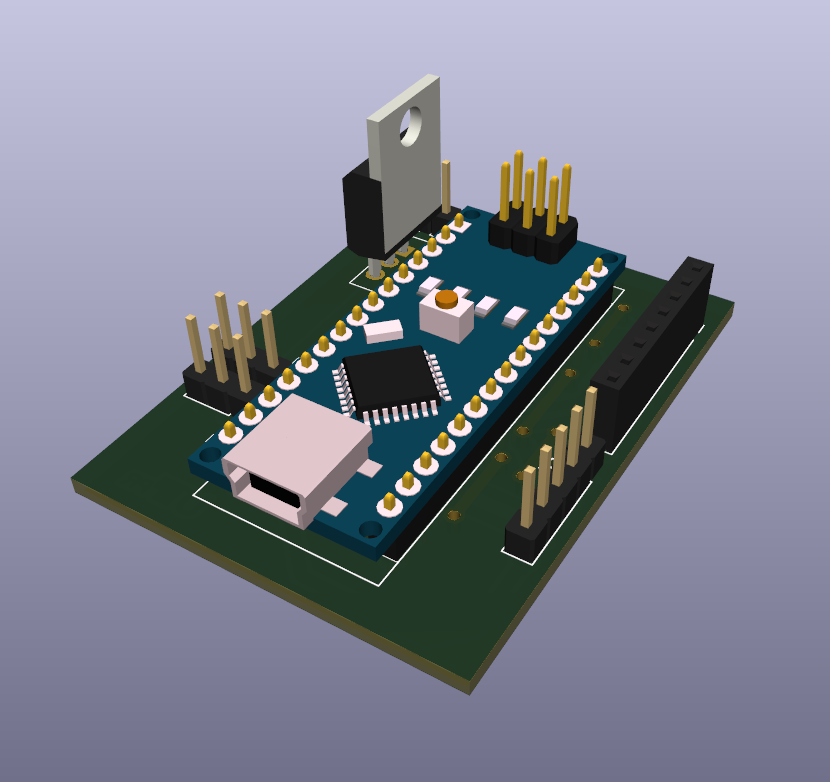
\includegraphics[width=0.6\textwidth]{Capitulo2 - Hardware/3D placa.PNG}\\
\caption{\label{fig:widgets}Modelo 3D da placa de circuito impresso.}
\end{figure}

\begin{figure}[H]
\centering
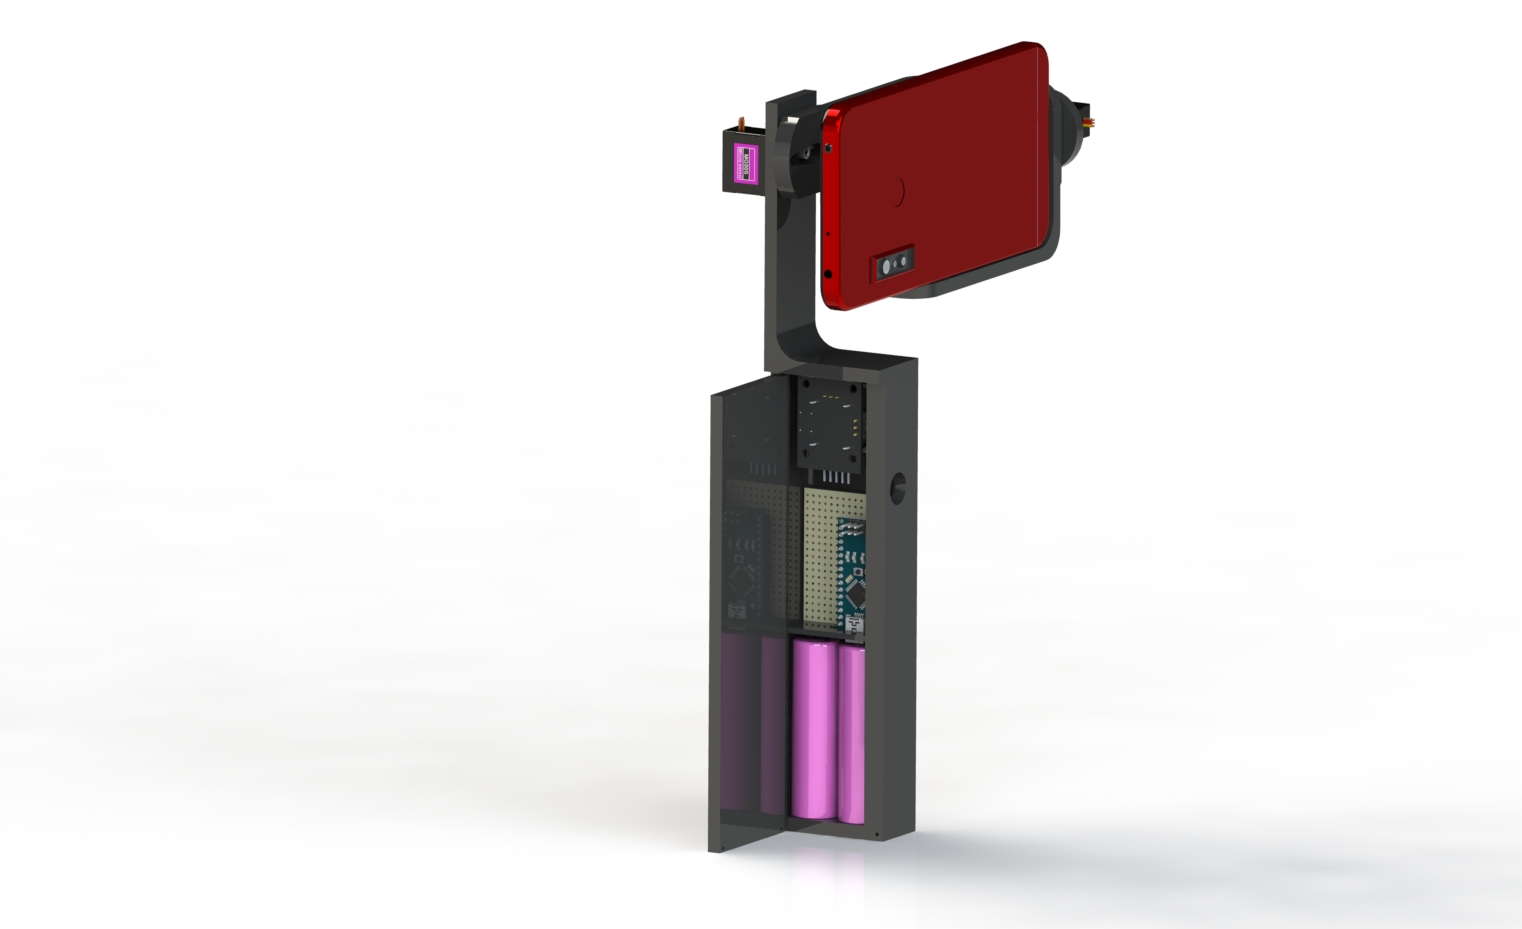
\includegraphics[width=0.6\textwidth]{Capitulo2 - Hardware/versao final.JPG}\\
\caption{\label{fig:widgets}Modelo 3D do dispositivo.}
\end{figure}


\section{Suporte articulado}
A estabilização para o equipamento preso à estrutura articulada é dada por dois eixos de rotação, estes possibilitam variar a inclinação do suporte na vertical e na horizontal de zero a 90 graus para cada lado, isto devido a cada servo motor MG90s possibilitar uma rotação de 180 graus. Cada servo motor opera entre 4,8 e 6 volts, com seu torque e velocidade de operação variando de acordo com esses parâmetros. Para um funcionamento estável, os motores não são alimentados pelo arduino, a tensão máxima fornecida aos dois servos é de 5 volts, como a tensão de saída do conjunto de baterias é de 7,2 volts, foi utilizado um regulador de tensão LM7805, que mantém uma tensão estável de 5 volts se a tensão de entrada for maior que 7 volts, não excedendo 30 volts, isso nos dá os parâmetros da tabela 2.

\begin{table}[H]
\centering
\begin{tabular}{j|j|j}
Tensão de entrada & Torque & Velocidade de operação \\\hline
4,8 & 1,8kg/cm & 0.1sec/60 graus\\
5,0 & 1,9kg/cm & 0.1sec/60 graus\\
6,0 & 2,2kg/cm & 0.08sec/60 graus\\
\end{tabular}
\caption{\label{tab:widgets}Tabela de parâmetros do servo motor MG90s para diferentes tensões de entrada.}
\end{table}

Ambos os servos são fixados diretamente na estrutura impressa por meio de dois parafusos, e as peças móveis da estrutura articulada são encaixadas diretamente no eixo de cada um dos servos com o auxilio de hélices de plástico. Para facilitar a movimentação das partes móveis e diminuir o atrito, e por consequência o desgaste do material plástico, foi adicionado sob cada eixo (encontro de duas partes móveis) duas arruelas de ferro com graxa. O cabeamento dos dois servos segue presa às estruturas móveis da estrutura articulada, isso devido ao comprimento necessário dos cabos ser diferente para diferentes posições de operação.


\section{Eletrônica}
%incluir esquematico, diagrama de blocos
O sistema conta com duas células (baterias) recarregáveis de 3,6 volts e 3000 mAh ligadas em série, fornecendo ao sistema 7,2 volts, este conjunto de baterias é ligado a um interruptor, e este é ligado à placa de circuitos. A trilha positiva se liga ao regulador de tensão LM7805 (que manda cerca de 5,0 volts aos dois servo motores), e também ao arduino nano (este não precisa de um regulador de tensão externo, como no caso dos dois servos, pois já possui um integrado em sua placa). O joystick analógico e o sensor MPU-6050 são conectados exclusivamente ao arduino conforme pode ser visto na figura 3. Todos os componentes são conectados por meio de barramentos soldados na placa, permitindo o funcionamento como pode ser visto na figura 4, dando ao sistema modularidade, uma vez que cada componente pode ser removido individualmente, facilitando operações como manutenção e ajustes.

\begin{figure}[H]
\centering
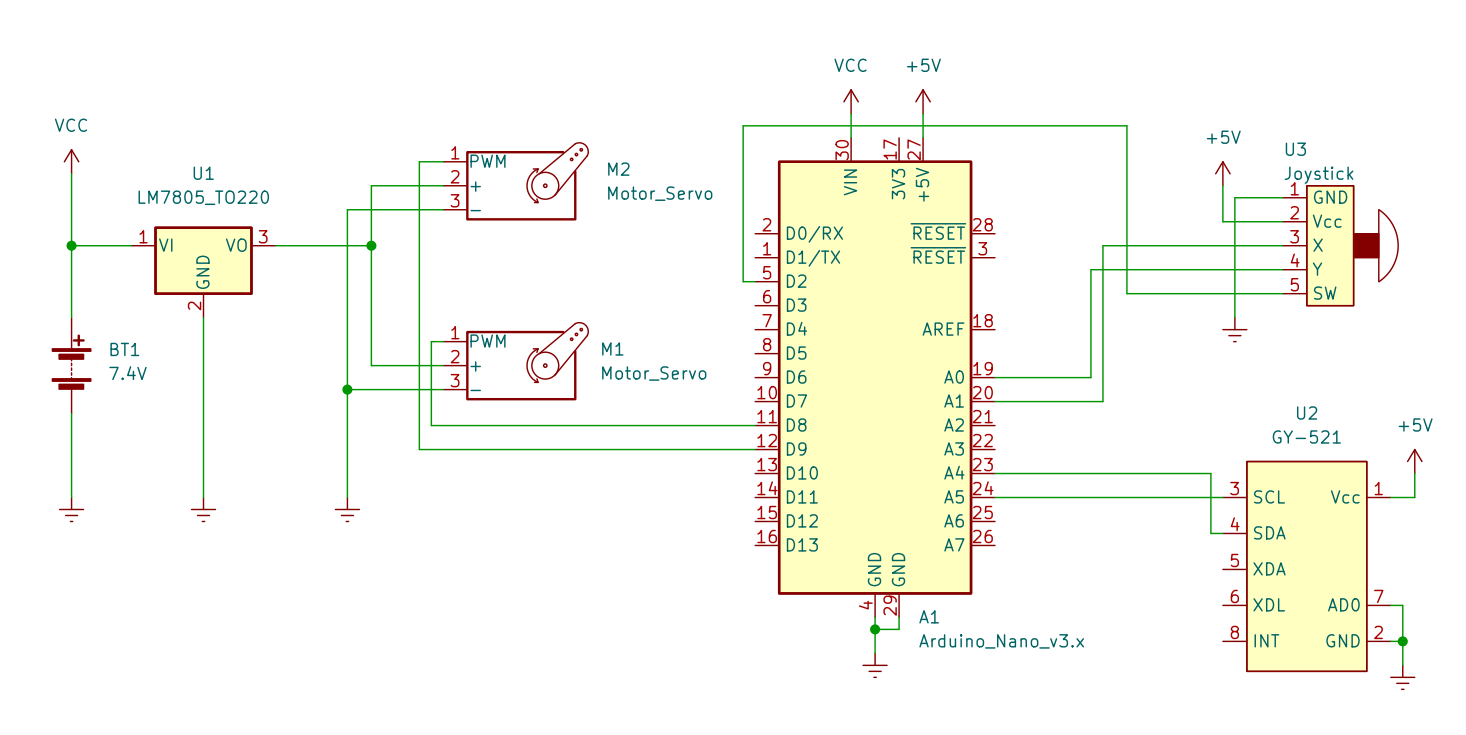
\includegraphics[width=0.9\textwidth]{Capitulo2 - Hardware/Esquematico.PNG}\\
\caption{\label{fig:widgets}Esquemático dos componentes eletrônicos.}
\end{figure}

\begin{figure}[H]
\centering
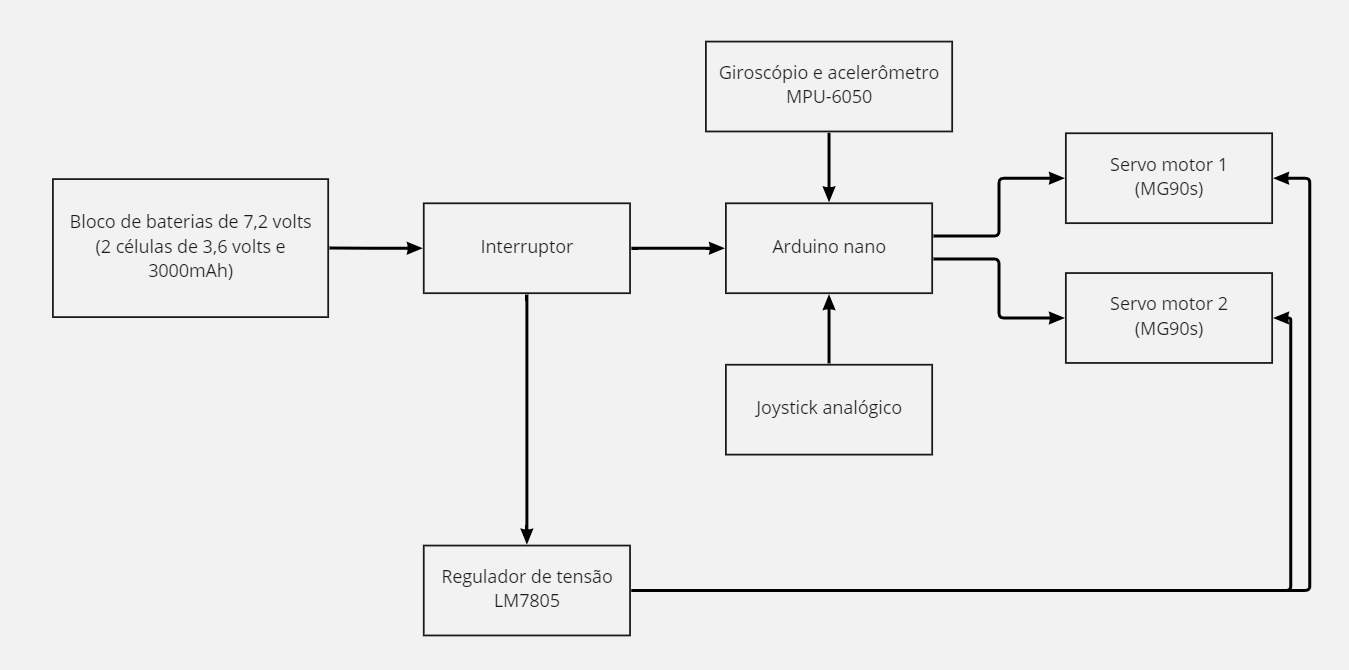
\includegraphics[width=0.9\textwidth]{Capitulo2 - Hardware/DiagramaDeBlocos.png}\\
\caption{\label{fig:widgets}Diagrama de blocos do dispositivo.}
\end{figure}


A placa de circuitos foi produzida manualmente pelos integrantes do grupo deste trabalho utilizando percloreto de ferro. A imagem do circuito foi produzida através do software KiCad, como pode ser visto na figura 5, e foi transferida de um papel fotográfico para a placa de fenolite utilizando uma fonte de calor, depois de resfriada, foi imersa em percloreto de ferro por cerca de cinco minutos. Após o fim do processo, obtivemos uma placa funcional do circuito do projeto, como pode ser visto na figura 6.

\begin{figure}[H]
\centering
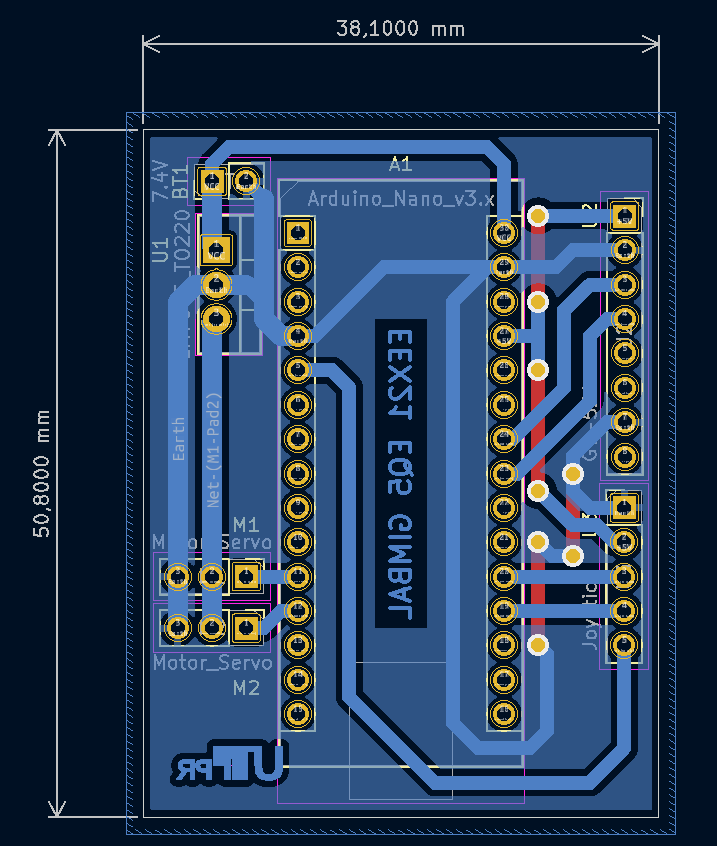
\includegraphics[width=0.5\textwidth]{Capitulo2 - Hardware/Circuito placa desenho.PNG}\\
\caption{\label{fig:widgets}Desenho do circuito no software KiCad.}
\end{figure}

\begin{figure}[H]
\centering
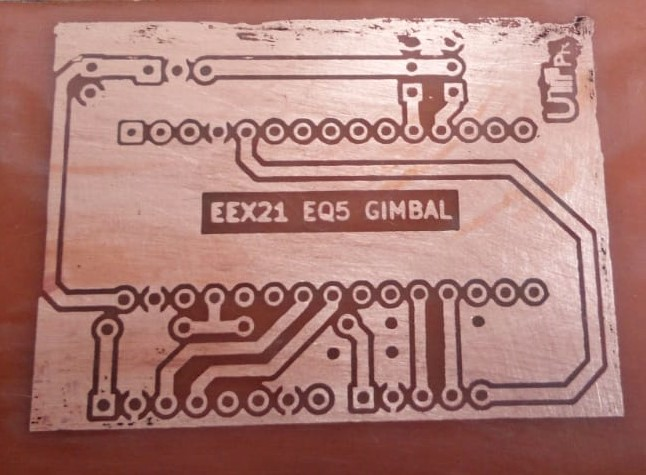
\includegraphics[width=0.5\textwidth]{Capitulo2 - Hardware/CircuitoPlaca.jpeg}\\
\caption{\label{fig:widgets}Placa produzida manualmente utilizando o processo de corrosão por percloreto de ferro.}
\end{figure}

Com exceção dos servo motores, os componentes são posicionados dentro da estrutura impressa (caixa) através de pequenos parafusos, dando espaço ao posicionamento do módulo MPU-6050 com sua placa orientada na horizontal, nos permitindo obter leituras precisas da inclinação nos dois eixos de rotação da estrutura articulada, como também possibilitar a passagem dos cabos sem prejudicar outros componentes. 